\chapter{The Temporal Context Model}\label{sec:tcm}
The temporal context model (TCM) was proposed by \textcite{Howard2002} as a model of free recall.
It matched data of immediate, delayed, and continuous distractor recall tasks.
As the distractor task used in the delayed and continuous distractor condition is designed to prevent active rehearsal, this model is likely to address more long-term, synaptic storage as opposed to the short-term OSE model.
Similar to a number of other memory models, the TCM assumes a time varying context signal that items are associated with.
But unlike those other models, this context is based on the items itself rather than being randomly generated.

In particular, items in the TCM are represented as orthogonal vectors $\tcmitem_i$ and the context signal is also a vector $\ctx$.
When we relax the orthogonality constrained on the items to almost orthogonal, we can use Semantic Pointers for these vectors.
To associate items and contexts, two association matrices are used.
The $\mtf$ matrix represents the associations from a context to an item and is constructed as an outer product matrix as
\begin{equation}
    \mtf = \sum_i \tcmitem_i \ctx_i\Tr \text{.}
\end{equation}
Note that the $\mtf$ matrix can easily be updated by adding another item/context outer product.
The $\mft$ matrix is used to retrieve a context vector $\ctxin_i = \mft \tcmitem_i$ to update the current context according to the \emph{evolution equation} (also see \cref{fig:tcm}a)
\begin{equation}
    \ctx_i = \theta_i \ctx_{i-1} + \tcmbeta \ctxin_i\label{eqn:ctx-update}
\end{equation}
where $\tcmbeta$ is a free parameter controlling how fast the context drifts and $0 < \theta_i \leq 1$ is determined to ensure unit length of $\ctx_i$ in each timestep as
\begin{equation}
    \theta_i = \sqrt{1 + \tcmbeta^2 \sbr{\left\langle\ctx_{i-1}, \ctxin_i\right\rangle^2 - 1}} - \tcmbeta \left\langle\ctx_{i-1}, \ctxin_i\right\rangle\text{.}
\end{equation}
In the CUE model, however, $\theta_i$ is fixed to the asymptotic value for $\langle\ctx_{i-1}, \ctxin_i\rangle \rightarrow 0$
\begin{equation}
    \theta_i = \sqrt{1 - \tcmbeta^2}\text{.}
\end{equation}
In the TCM this corresponds to the assumption that item $i$ has not been presented for a sufficiently long time which results in the a retrieved context $\ctxin_i$ that is almost orthogonal to the current context.
This change is further motivated by still producing a good match to the data and simplifying the neural implementation as no dynamic scaling of a vector is required which requires a product network for each vector dimension in the NEF\@.
\Cref{eqn:ctx-update} introduces the asymmetric bias to forward recall into the model (\cref{fig:ctxsim}).
While the similarity of contexts $\langle\ctx_i, \ctx_j\rangle$ is symmetric for the lag $j - i$, $\ctxin_i$ will only be included in context vectors $\ctx_j$ with $j \geq i$.
\begin{figure}
    \hfill
    \subcaptionbox{}{\begin{tikzpicture}[every path/.style={-Latex}]
        \graph [grow down=1.5cm, branch right=1.5cm] {
            f0/"$\tcmitem_{i-2}$" -> ["$\mft$" anchor=east] cin0/"$\ctxin_{i-2}$" -> ["$\tcmbeta$" anchor=east] c0/"$\ctx_{i-2}$";
            f1/"$\tcmitem_{i-1}$" -> cin1/"$\ctxin_{i-1}$" -> c1/"$\ctx_{i-1}$";
            f2/"$\tcmitem_{i}$" -> cin2/"$\ctxin_{i}$" -> c2/"$\ctx_{i}$";
            start/"$\dots$" [x=-6cm, y=-3cm] -> ["$\theta$" below] c0 -> c1 -> c2 -> end/"$\dots$" [y=-1.5cm];
        };
    \end{tikzpicture}}  % chktex 31
    \hfill
    \subcaptionbox{}{\begin{tikzpicture}[every path/.style={-Latex}]
        \graph [grow down=1.5cm, branch right=1.5cm] {
            start/"$\dots$";
            c0/"$\ctx_i$" -> ["$\mtf$" anchor=east] f0/"$\tcmitemin_i$" -> ["$\mft$" anchor=east] cin0/"$\ctxin_i$";
            c1/"$\ctx_{i+1}$" -> f1/"$\tcmitemin_{i+1}$" -> cin1/"$\ctxin_{i+1}$";
            c2/"$\ctx_{i+2}$" -> f2/"$\tcmitemin_{i+2}$" -> cin2/"$\ctxin_{i+2}$";
            cin0 -> ["$\tcmbeta$" {near end, yshift=-3mm}] c1;
            cin1 -> c2;
            start -> c0 -> ["$\theta$"] c1 -> c2 -> end/"$\dots$";
            cin2 -> end;
        };
    \end{tikzpicture}}  % chktex 31
    \hfill
    \caption{Evolution of the context in the TCM during (a) item presentation and (b) recall.}\label{fig:tcm}
\end{figure}
\begin{figure}
    \centering
    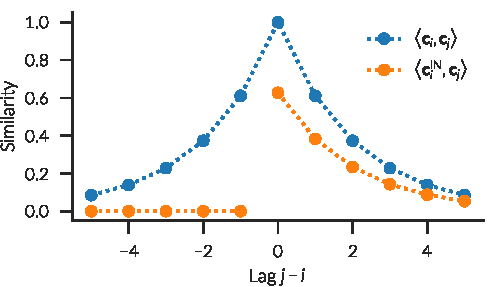
\includegraphics{figures/ctxsim}
    \caption{Similarity of the context to itself $\langle \ctx_i, \ctx_j \rangle$ and to the retrieved context $\langle \ctxin_i, \ctx_j \rangle$ for different lags $j-i$.}\label{fig:ctxsim}
\end{figure}

Finally, the associations from items to context $\mtf$ need to be updated, so that a recalled item can be used to update and partially restore a previous context to retrieve further items.
In the original TCM, this update is given by
\begin{align}
    \mft_{i+1} &= \mft_i \tilde{\mat{P}}_{\tcmitem_i} + a_i \mft_i \mat{P}_{\tcmitem_i} + b_i \ctx_i \tcmitem_i\Tr \\
    a_i &= \gamma b_i \\
    b_i &= \frac{1}{\gamma^2 + 2 \gamma \left\langle\ctxin, \ctx_i\right\rangle + 1}
\end{align}
with projection operators $\mat{P}_{\vc v} = \vc v \vc v\Tr\!/ \norm{\vc v}^2$, $\tilde{\mat{P}}_{\vc v} = \imat - \mat{P}_{\vc v}$, and a free parameter $\gamma$ specifying the relative contribution of previously associated context $\ctxin_i$ and new context $\ctx_i$.
Again, to facilitate the neural implementation, the exact weighting of $\ctxin_i$ and $\ctx_i$ is relaxed while still achieving a good match to data.
Instead of splitting $\mft_i$ into components parallel and orthogonal to $\tcmitem_i$, $\ctx_i\tcmitem_i\Tr$ is added directly into the matrix with a fixed parameter $b$,
\begin{equation}
    \mft_{i+1} = \mft_i + b \ctx_i\tcmitem_i\Tr\text{.}
\end{equation}

Given a context $\ctx$ a mixture of associated items can be recalled as $\tcmitemin = \mtf \ctx$.
To retrieve a single item some form of cleanup as to performed.
Once such a single item has been recalled, the item can be used to recall the associated context as $\mft \tcmitemin$ which in turn can be used to update the current context according to \cref{eqn:ctx-update}.
The updated context allows than to recall further item (\cref{fig:tcm}b).

Different cleanup strategies for the recalled item vector can be used.
In the original TCM model, a set of activities $a_i = \tcmitem_i\Tr \tcmitemin$ was obtained and used to make a probabilistic decision according to Luce's choice rule.
The probability of retrieving item $\tcmitem_i$ is given as
\begin{equation}
    P\bigl(\tcmitem_i \bigl|\,\tcmitemin\bigr) = \frac{\exp\!\del{\frac{2a_i}{\tau}}}{\sum_j \exp\!\del{\frac{2a_j}{\tau}}}
\end{equation}
with a parameter $\tau$ that specifies the sensitivity to the activities.

The version of the TCM model presented by \textcite{Sederberg2008}, uses a winner-take-all process based on the leaky, competing accumulator model \parencite{Usher2001}.
In this model, for each possible item a leaky integrator integrates evidence over time.
At the same time, the integrators inhibit each other laterally.
The dynamics can be described by
\begin{equation}
    \vc x_s = \vc x_{s - 1} + \frac{1}{\tau} \del{\vc u - \kappa \vc x_{s - 1} - \lambda \mat L \vc x_{s - 1}} + \vc\eta
\end{equation}
where $\vc u$ is the scaled vector of inputs determined from $\mtf \ctx$ from the current context, $\kappa$ the leak rate, $\lambda$ the lateral inhibition, ${[\mat L]}_{ij} = 1 - \krond_{ij}$ the lateral inhibition matrix, and $\vc\eta$ normal distributed random noise.
This is a more detailed description of how the brain might actually decide for a single item.
However, it is problematic to integrate within a larger scale neural model under noisy conditions as detailed in \cref{sec:recall}.
For this reason, a different winner-take-all all process described in the same chapter will be used.
